% Created 2021-10-13 Wed 20:24
% Intended LaTeX compiler: pdflatex
\documentclass[11pt]{article}
\usepackage[utf8]{inputenc}
\usepackage[T1]{fontenc}
\usepackage{graphicx}
\usepackage{grffile}
\usepackage{longtable}
\usepackage{wrapfig}
\usepackage{rotating}
\usepackage[normalem]{ulem}
\usepackage{amsmath}
\usepackage{textcomp}
\usepackage{amssymb}
\usepackage{capt-of}
\usepackage{hyperref}
\author{190022658}
\date{\today}
\title{CS3104 System Utility - Report}
\hypersetup{
 pdfauthor={190022658},
 pdftitle={CS3104 System Utility - Report},
 pdfkeywords={},
 pdfsubject={},
 pdfcreator={Emacs 27.2 (Org mode 9.5)}, 
 pdflang={English}}
\begin{document}

\maketitle

\section{Overview}
\label{sec:orgbe92360}
In this practical, we were required to use linux system calls to implement a system utility similar to \texttt{ls -n}. The \texttt{ls -n} implementation also produces an output that has a green color for directories.

\begin{itemize}
\item Implemented the \texttt{ls -n} command
\item Implemented the \texttt{cat} command
\end{itemize}


\section{Design}
\label{sec:orgd32be05}
\subsection{System Calls (inline asm)}
\label{sec:org9e08fd3}
\begin{itemize}
\item System calls hold parameters in registers.
\item The return value is stored in the eax register.
\item The system call number goes in the eax register, the first argument in edi, the second in esi and the third in edx. There are 6 registers in total as in the first link below.
\item Same is true in for the shortcut used in the code.
\item There are constraints to force the variable into the specific registers.

\item \url{https://en.wikibooks.org/wiki/X86\_Assembly/Interfacing\_with\_Linux\#System\_calls}
\end{itemize}

\subsection{ls implementation}
\label{sec:org5f5936a}
\begin{description}
\item[{\_strlen(char*)}] calculates the length of char array. Places a char pointer to the end of the array ('$\backslash$0') and subtracts the pointer placed at the beginning of the array.
\item[{print(char*)}] uses the write system call and passes the char array length as the third argument by using the \_strlen function.
\item[{myopen(char*)}] uses the open system call and passes the arguments using the registers.
\item[{mystat(char*, struct stat)}] uses the stat system call and passes the arguments using the registers.
\item[{mygetdents(int, char*, int)}] uses the getdents system call and passes the arguments using the registers.
\item[{intToString(int)}] returns a char*. Here I declare a static character array (otherwise if a function returns a char* it becomes a dangling pointer) and a char pointer which points towards the end of the array. Then I place a '$\backslash$0' at the end to show that it ends there. Then using a while loop, I do a number \% 10 and place that where the pointer points and decrement the pointer and divide the number by 10. This is done till the number is not 0. After this the pointer will be pointing towards the beginning of the string and so I return the pointer. This function will not and is not supposed to work to store the result. For example -
\begin{verbatim}
    char* fifty = intToString(50);
    print(intToString(500));
    print("\n");
    print(fifty);
    // Output
    // 500
    // 00
\end{verbatim}
\item[{printInt(int)}] converts the int to a string using the intToString function and prints it.
\item[{printIntWithSpaces(int, int)}] prints (numberofspaces - length of number as a string) spaces then prints the number. This is for beautiful formatting. The other option was using '\t' but that was not working out so well.
\item[{printTime(struct tm time)}] prints out the time using the fields of the struct as wanted.
\item[{printDetails(char*, char*)}] uses the stat system call to get the stat struct's value. And uses that to print out the details needed. The one thing to notice is that I noticed the difference between the masks for st\textsubscript{mode} in the inode's man page. That's why I used the '>>' operator to shorten the code. Another thing is that I print in different color when it's a directory name.
\item[{printRelativeDir(char*, char*)}] this basically takes two paths and joins them. For example ``\textasciitilde{}/Documents'' and ``something.txt'' will become ``\textasciitilde{}/Documents/something.txt''. Notice the '/' that has been added. After this the printDetails function is called.
\item[{ls(char*)}] calls the mystat function for the char array. If it's a file then it calls the printDetails function for it, if its a directory then uses myopen and mygetdents. Then as shown in the example in the man page for getdents, using a struct linux\textsubscript{dirent} pointer iterate through the directory and call the printRelativeDir function for the file name.
\end{description}
\subsection{cat implementation}
\label{sec:org323205f}
Uses the open, read and write system calls
\begin{description}
\item[{\_strlen(char*)}] same as before
\item[{print(char*)}] same as before
\item[{myopen(char*)}] same as before
\item[{myread(int, char*, int)}] uses the read system call
\item[{readandwrite(int)}] takes file descriptor as argument. Uses myread to read the contents of file and writes it out using the print function.
\item[{main(int, char**)}] if no argument then uses standard input as file descriptor. Otherwise opens the file given as argument.
\end{description}


\section{Testing}
\label{sec:org51dcefa}
There's a test.sh file that aims to replicate the result for ls.
\subsection{ls}
\label{sec:org6e01d4c}
\begin{verbatim}
./ls myls.c
-rw-r--r--    1 1000 1000   5516 Oct 13 17:40 myls.c

./ls
-rw-r--r--    1 1000 1000   5516 Oct 13 17:40 myls.c
-rw-r--r--    1 1000 1000   1666 Oct 13 19:21 mycat.c
-rw-r--r--    1 1000 1000    359 Oct 13 17:40 Makefile
-rwxr-xr-x    1 1000 1000    165 Oct 13 19:39 test.sh
-rwxr-xr-x    1 1000 1000  21720 Oct 13 19:27 ls
-rwxr-xr-x    1 1000 1000  18200 Oct 13 19:27 cat
total 64

./ls .
-rw-r--r--    1 1000 1000   5516 Oct 13 17:40 myls.c
-rw-r--r--    1 1000 1000   1666 Oct 13 19:21 mycat.c
-rw-r--r--    1 1000 1000    359 Oct 13 17:40 Makefile
-rwxr-xr-x    1 1000 1000    165 Oct 13 19:39 test.sh
-rwxr-xr-x    1 1000 1000  21720 Oct 13 19:27 ls
-rwxr-xr-x    1 1000 1000  18200 Oct 13 19:27 cat
total 64

./ls ./
-rw-r--r--    1 1000 1000   5516 Oct 13 17:40 myls.c
-rw-r--r--    1 1000 1000   1666 Oct 13 19:21 mycat.c
-rw-r--r--    1 1000 1000    359 Oct 13 17:40 Makefile
-rwxr-xr-x    1 1000 1000    165 Oct 13 19:39 test.sh
-rwxr-xr-x    1 1000 1000  21720 Oct 13 19:27 ls
-rwxr-xr-x    1 1000 1000  18200 Oct 13 19:27 cat
total 64

./ls ..
drwxr-xr-x    1 1000 1000      0 Sep 27 23:11 Lectures
-rw-r--r--    1 1000 1000  98506 Sep 27 23:11 P1-SystemUtility.pdf
-rw-r--r--    1 1000 1000   5270 Sep 27 23:11 faq.txt
drwxr-xr-x    1 1000 1000     20 Sep 27 23:15 temp
drwxr-xr-x    1 1000 1000     66 Oct 13 19:29 src
drwxr-xr-x    1 1000 1000     20 Oct 12 16:38 report
total 108

./ls /
drwxr-xr-x    1 0 0    124 Oct  2 19:00 var
drwxr-xr-x   21 0 0   4420 Oct  4 18:32 dev
drwxr-xr-x   23 0 0    600 Oct 13 10:04 run
drwxr-xr-x    1 0 0   2416 Oct 13 10:04 etc
drwxrwxrwx   15 0 0    880 Oct 13 19:40 tmp
dr-xr-xr-x   13 0 0      0 Oct  2 19:00 sys
dr-xr-xr-x  282 0 0      0 Oct  2 19:00 proc
drwxr-xr-x    1 0 0     80 Oct 12 19:51 usr
drwxr-xr-x    1 0 0  49992 Oct 12 19:51 bin
drwxr-xr-x    1 0 0    134 Oct 11 13:58 boot
drwxr-xr-x    1 0 0     12 Jul  7 19:35 home
drwxr-xr-x    1 0 0  91500 Oct 12 19:51 lib
drwxr-xr-x    1 0 0  91500 Oct 12 19:51 lib64
drwxr-xr-x    1 0 0      0 May 31 01:39 mnt
drwxr-xr-x    1 0 0     14 Sep 24 10:42 opt
drwxr-x---    1 0 0    100 Sep 25 20:47 root
drwxr-xr-x    1 0 0  49992 Oct 12 19:51 sbin
drwxr-xr-x    1 0 0     14 Sep 10 10:03 srv
drwxr-xr-x    1 0 0    156 Sep 27 14:03 snap
total 16

./ls dakjdfh
No such regular file or directory
\end{verbatim}

\begin{figure}[htbp]
\centering
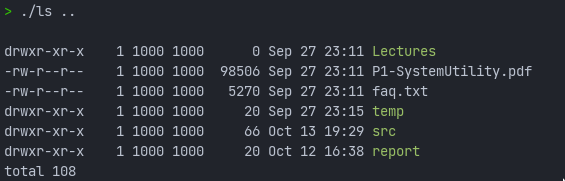
\includegraphics[width=.9\linewidth]{./color-ls.png}
\caption{\label{colorls}The directory names have green color}
\end{figure}

\subsection{cat}
\label{sec:orgb43725e}


\section{Evaluation}
\label{sec:org1a8bc69}
The output for the total is below and not at the top as in \texttt{ls -n}. To put this on the top I would have to iterate the directory twice. Then I saw that the example in the practical specification did not have a total field, so I didn't iterate twice.

\section{Conclusion}
\label{sec:org1dbe88c}
In the practical, I learn about system calls. I also gained experience of system level programming.
\end{document}
